\section{What We Discovered}
\label{sec:results}



We run the experimental process from section~\ref{sec:rational} on the
sampled debugging scenarios from section~\ref{sec:sample} using a machine with two Intel Xeon Gold 6258R processors and 500GB of memory.
Each debugging scenario had a timeout limit of 4 minutes and a
memory limit of 6GB. The complete experiment required
over 30,000 hours of compute hours on our machine.


Figure~\ref{fig:avo-matrix} summarizes our results and provides answers to
the four questions from section~\ref{subsec:experiment}.  Specifically, it
depicts a head-to-head comparison of the usefulness of each mode against
every other mode.  The cell in row $R$ and column $C$ plots the percentage
of interesting debugging scenarios for which $R$ is more useful $C$ ---
this percentage has been calculated as an estimated proportion from the
corresponding proportion of the debugging scenarios in our sample and the
upper bound.  In effect, reading across a given row $R$ provides an
overview of how $R$ compares to every other mode; the higher the bars, the
more interesting debugging scenarios for which $R$ is strictly more useful
than the other modes.  Reading down a given row $C$ provides an overview
of how every other mode compares to $C$; the higher the bars, the more
interesting debugging scenarios for which $C$ is strictly less useful than
the other modes. For example, the second cell in the row of Natural blame
shows that Natural is more useful than Natural exceptions for 12\% of all
the interesting debugging scenarios we generate from our benchmarks and
mutators. 

Figure~\ref{subsec:experiment} shows that the answers for questions $Q_1$
to $Q_3$ are positive. In all three semantics, blame modes outperform
their corresponding exception mode (by 9.44\% to 12.7\%). The Natural
exceptions mode is never more useful than Natural blame, and  Transient
exceptions are more useful than Transient first and Transient last blame
in 2.19\% and 2.8\% of the scenarios respectively. 


For the answers to $Q_*$, we compare the percentages in antisymmetric
positions in the matrix. Blame for all three semantics is significantly
more useful than Erasure exceptions (by 33\% to 35\%). Natural blame is
more useful than both versions of Transient blame by a small percentage;
in 4.05\% of scenarios Natural blame is more useful while in 1.67\% of the
scenarios Transient blame is more useful. The Transient first and
Transient last blame are practically indistinguishable. Finally, there is
no clear winner between Natural exceptions and Transient exceptions
despite the theoretically advantageous additional checks of the Natural
semantics.

\begin{figure}
  \centering
  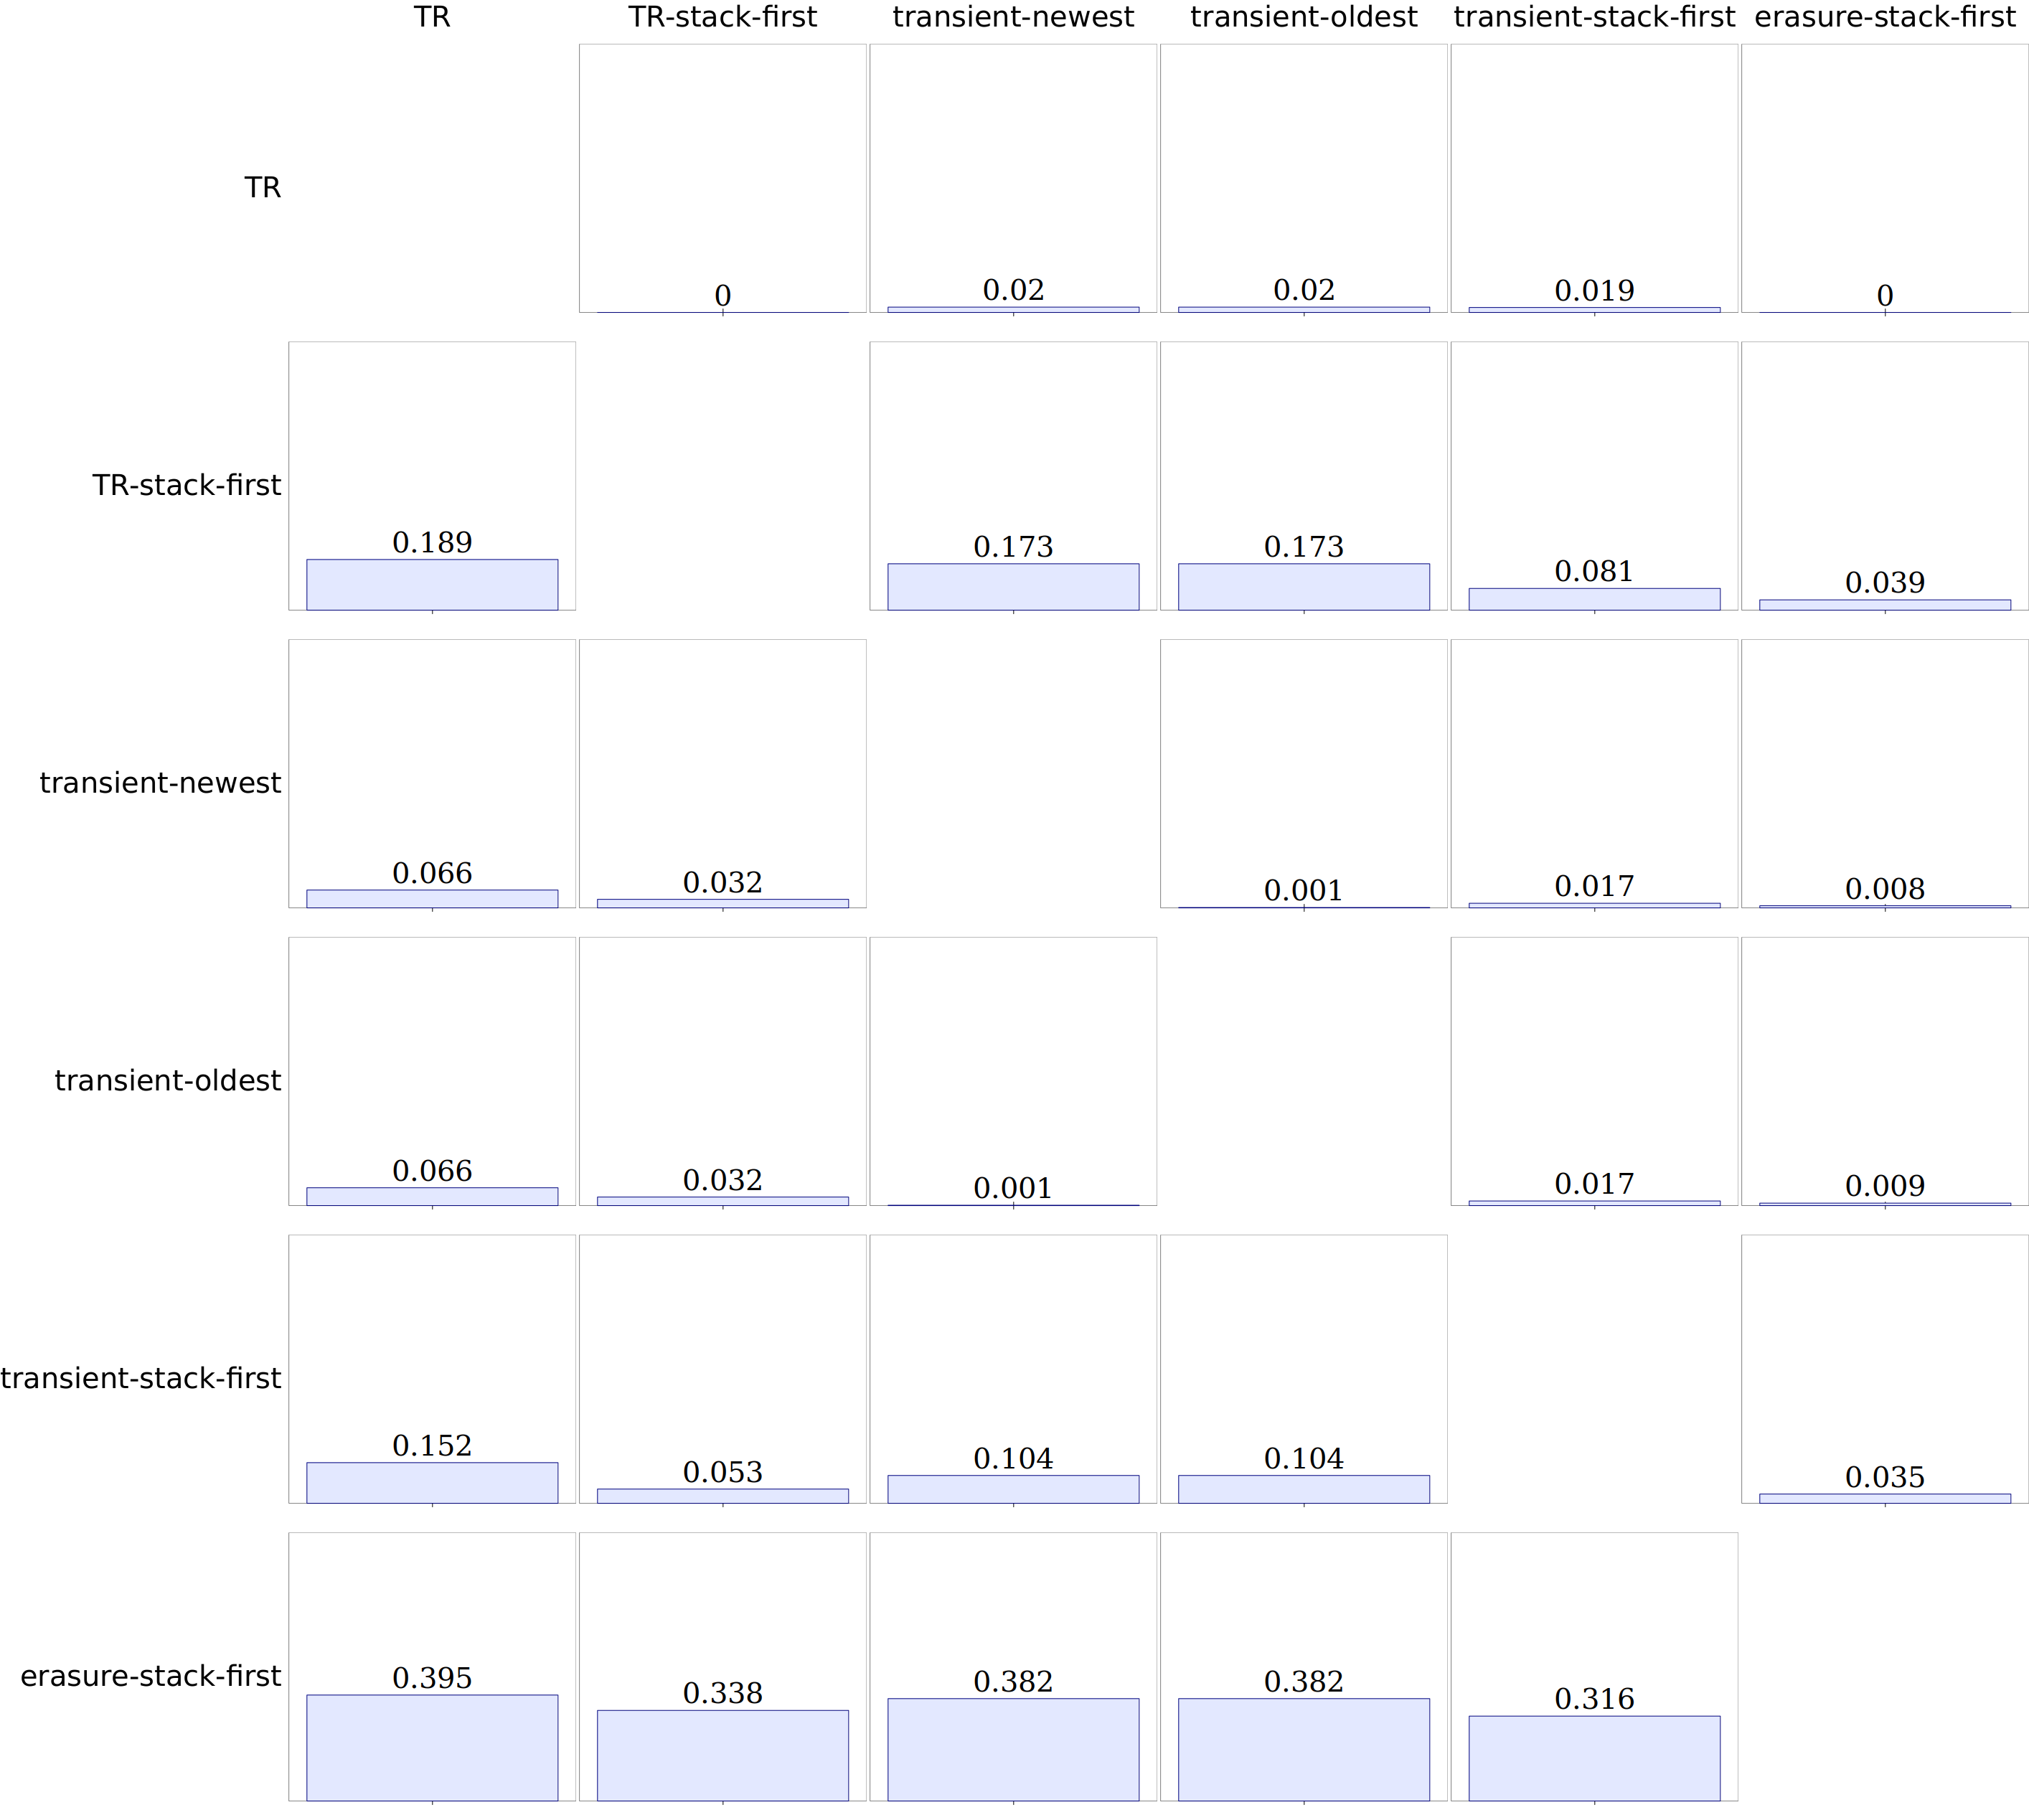
\includegraphics[width=0.45\textwidth]{./plots/avo-matrix}
  \caption{Usefulness comparisons: Each cell depicts the estimated percentage of
  interesting debugging scenarios for which the row mode is more useful
  than the column mode.
  The upper bound of error margin is 0.02\%}
  \label{fig:avo-matrix}
\end{figure}


\begin{figure}
  \centering
  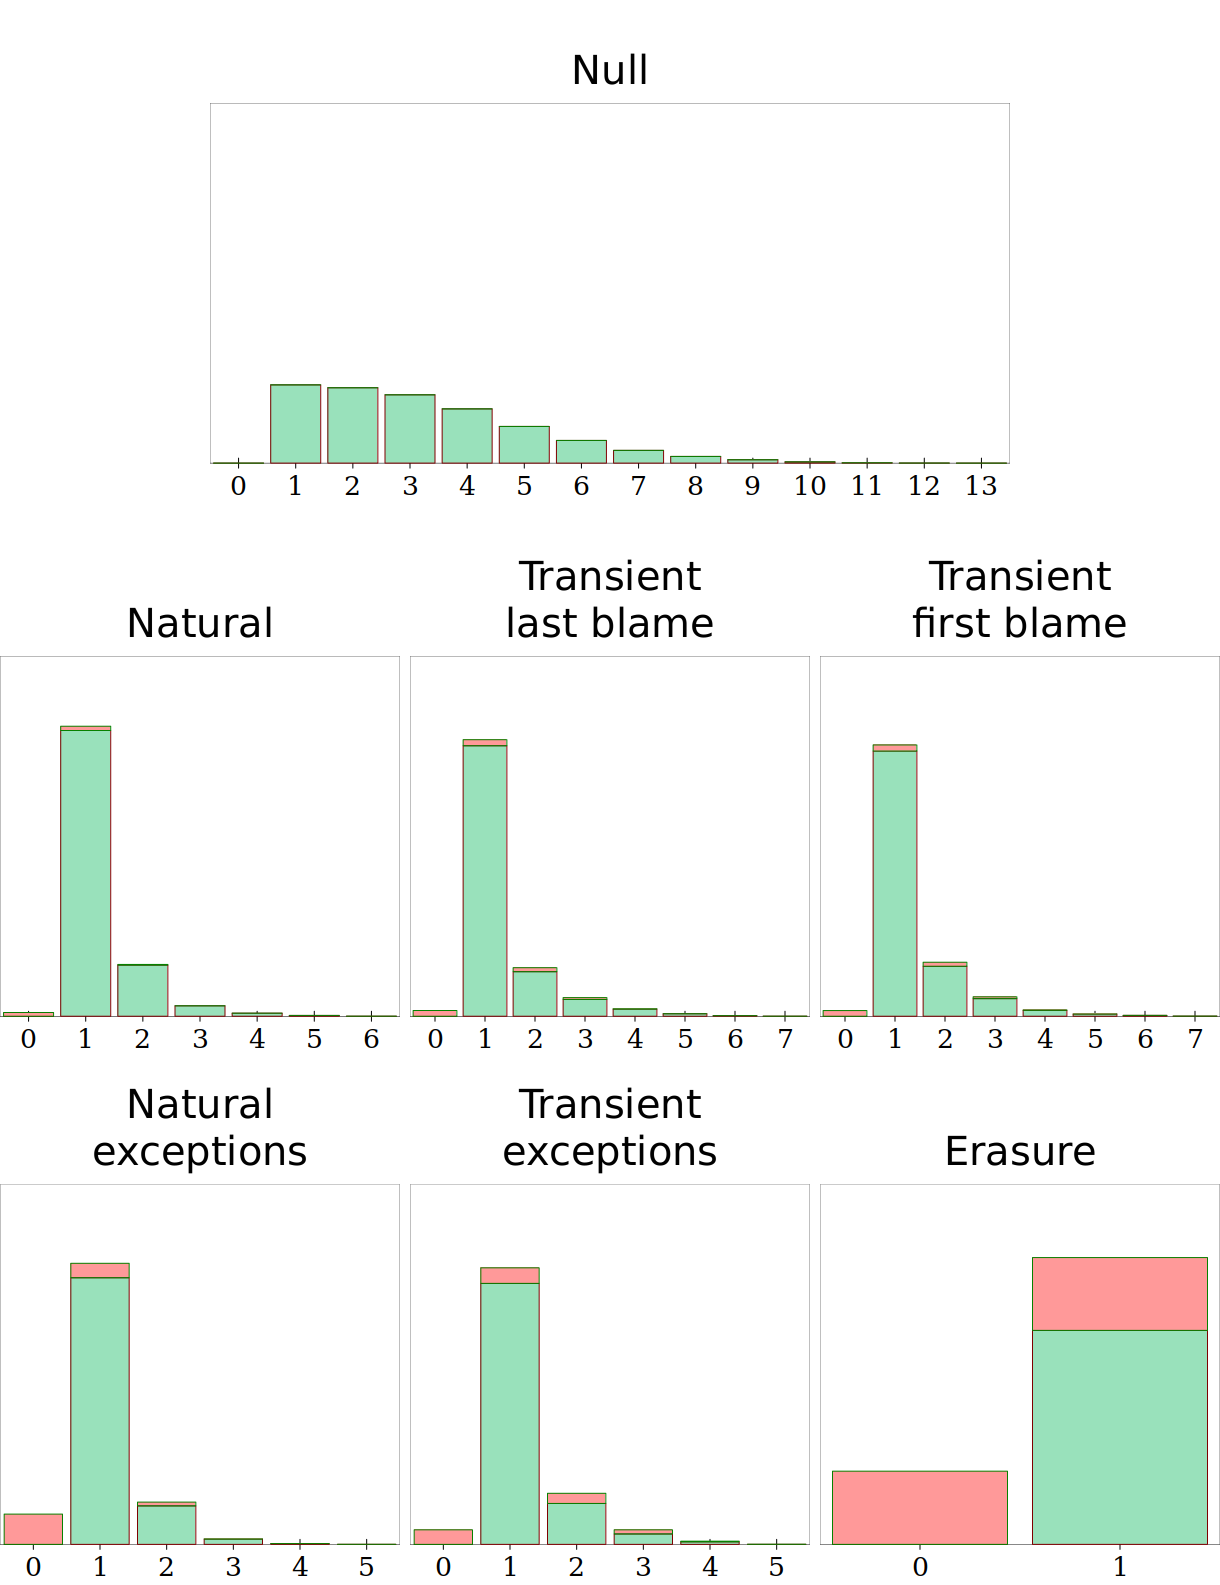
\includegraphics[width=0.4\textwidth]{./plots/bt-lengths-table}
  \caption{Programmer effort: Each plot depicts the distribution of trail
  lengths for a given mode across all benchmarks, starting from trails
  of length 0.}
  \label{fig:effort-table}
\end{figure}


Figure~\ref{fig:effort-table} shows the distribution of programmer effort
for our sample of interesting debugging scenarios. Unlike the usefulness
comparisons above, these proportions do not generalize to a representation of the full population.
Still, as we discuss in section~\ref{subsec:effort}, they provide an
alternative view of the workings of the rational programmer. 

There are
three immediate take-aways from the figure. First, the effort for successfully
debugging interesting scenarios (in green) for the random mode of the
rational programmer follows  a normal distribution, as expected.\footnote{The
random mode distribution is indistinguishable for all three semantics and thus the figure~\ref{fig:effort-table} 
only shows one plot.} In contrast, in the other modes, successful effort coalesces at
the left side of the plot, meaning that in most cases the programmer needs
to type a single component to debug a scenario. 

A second point of interest is that the exceptions of
the Erasure semantics either help the rational programmer immediately or 
the rational programmer fails to debug a scenario altogether (in red).
This is expected; no matter how many type annotations the programmer
adds to an Erasure program, if the type checker doesn't reject the
program, running the program always produces the same outcome. Thus an
exception from the runtime has to point to the buggy module with
the first try. Otherwise the rational programmer types an irrelevant
module, runs the program again and the exception points again to the
already typed module. 

A third notable piece of information from
the figure is that every mode has failed debugging scenarios, not just
Erasure. This should
not come as a surprise to the astute
reader. After all, as we
discuss above, some modes are more successful than others in certain
scenarios. Indeed any mode can fail if running a scenario results in an
exception and the exception carries no useful information about which
module the programmer should type next, e.g., because the stack trace 
does not contain frames from any module of the program, or only typed modules. This situation
can even happen immediately, which explains failures with 0 effort. 


While most failures to debug scenarios follow the above pattern, a few do not.
Breaking down the reasons for failure for Natural blame (1748 in total)
reveals an additional cause. For a small set of
debugging scenarios (40), Natural produces a run time type error
blaming a non-buggy already typed
component. We tracked down all these cases to known open issues with Typed
Racket and class contracts. 

In Transient, similar to Natural,
most failures are due to unhelpful exception information (1851 for both
Transient first and last blame).  
However, Transient also has a substantial
number of failures because scenarios hit the time and memory
limits of our experiment (~ 770 scenarios).  Additionally, there are nearly a 1000 cases where
Transient reports an empty blame set which leaves the rational programmer
without hints about how to proceed.
In~\ref{sec:threat:transient}, we discuss how both of these causes of
failure for Transient affect our experiment. 

